\documentclass{article}   	                         % use "amsart" instead of "article" for AMSLaTeX format
\usepackage{fullpage}                		% ... or a4paper or a5paper or ... 
\usepackage{enumerate}				% Use enumerate to list subsections
\usepackage{graphicx}				% Use pdf, png, jpg, or eps§ with pdflatex; use eps in DVI mode
\usepackage{fancyvrb}
\usepackage{amsmath}
\usepackage{dsfont}
\newcommand{\ra}{\rightarrow}

%SetFonts

\title{Computer System Fundamentals HW \#3}
\author{Quan Zhou}
\date{Feb 11th, 2016}
\begin{document}
\maketitle
\section*{Problem 1}
\begin{enumerate}[(a)]
\item
To find the standard deviation of the 40 sample:\\
\begin{equation}0.4 = z\left(\frac{\sigma}{\sqrt40}\right)\end{equation}
by looking up the table, $z = \Phi^{-1}(\Phi(z)) = \Phi^{-1}(0.96+0.02) = \Phi^{-1}(0.98) = 2.0537$
(note that $\alpha = 1 - 0.96 = 0.04$). So $\sigma = 1.23$
\item
For 99th percentile: $\alpha = 1- 0.99 = 0.01$. So $\Phi(z) = P(Z\leq z) = 1 - \frac{\alpha}{2} = 0.995$. By looking up the z-table, we found z = 2.57. Then we just need to find :\\
\begin{equation} \left[\bar X - z\frac{\sigma}{\sqrt n}, \bar X + z\frac{\sigma}{\sqrt n}\right]\end{equation}
so the 99th confidence interval is $\left[3 - 2.57\frac{1.23}{\sqrt 40}, 3 + 2.57\frac{1.23}{\sqrt 40}\right]$, or [3 - 0.50, 3 + 0.50] or [2.50, 3.50].
\item
So the new interval is [3 - 0.1, 3 + 0.1], or $z\frac{\sigma}{\sqrt n\prime} = 0.1$. We know z = 2.0537 just like in part (a), and $\sigma = 1.23$ as we found in (a). So the $n\prime = 160$. \\
So we need 120 more samples in order to narrow the confidence level at same $\alpha$.

\end{enumerate}

\section*{Problem 2}
\begin{enumerate}[(a)]
\item
SIMULATION 1: lambda = 60.0, Ts = 0.015, Sim length = 100.0\\
Results from M/M/1 Simulation\\
requests: 10852\\
w = 8  requests\\
q = 9  requests\\
Tw = 0.15315843087717834 sec\\
Tq = 0.16839097708418896  sec\\
Ts = 0.015161946764363964  sec\\
DONE.\\
compared with:\\
$$\rho = \lambda Ts = 0.9$$
$$q = \frac{\rho}{1-\rho} = 9$$
$$w = q-\rho = 9-0.9 = 8.1$$
$$T_q = \frac{q}{\lambda} = \frac{9}{60} = 0.15$$
$$T_w = \frac{w}{\lambda} = \frac{8.1}{60} = 0.135$$
Through there are some differences in the values, but for the most part, the simulation results are similar to the calculated results.\\
\item
SIMULATION 2: lambda = 50.0, Ts = 0.015, Sim length = 100.0\\
Results from M/M/1 Simulation\\
requests: 8016\\
w = 1  requests\\
q = 2  requests\\
Tw = 0.04654116499551064 sec\\
Tq = 0.061661745007644854  sec\\
Ts = 0.015120580012134389  sec\\
DONE.\\
compared with:\\
$$\rho = \lambda Ts = 0.75$$
$$q = \frac{\rho}{1-\rho} = 3$$
$$w = q-\rho = 3-0.75 = 2.25$$
$$T_q = \frac{q}{\lambda} = \frac{3}{50} = 0.06$$
$$T_w = \frac{w}{\lambda} = \frac{2.25}{60} = 0.0375$$
Through the simulated values are lower than the calculations, but for the most part, the simulation results are similar to the calculated results.\\
\item
SIMULATION 3: lambda = 65.0, Ts = 0.015, Sim length = 100.0\\
Results from M/M/1 Simulation\\
requests: 12881\\
w = 39  requests\\
q = 40  requests\\
Tw = 0.6043674892828412 sec\\
Tq = 0.6242865086817099  sec\\
Ts = 0.01509505164654915  sec\\
DONE.\\
compared with:\\
$$\rho = \lambda Ts = 0.975$$
$$q = \frac{\rho}{1-\rho} = \frac{0.975}{0.025} = 39$$
$$w = q-\rho = 39-0.975 = 38.025$$
$$T_q = \frac{q}{\lambda} = \frac{39}{65} = 0.6$$
$$T_w = \frac{w}{\lambda} = \frac{38.025}{65} = 0.585$$
Through the simulated values are higher than the calculations, but for the most part, the simulation results are similar to the calculated results.\\
\item
SIMULATION 4: lambda = 65.0, Ts = 0.02, Sim length = 100.0\\
Results from M/M/1 Simulation\\
requests: 13077\\
w = 1505  requests\\
q = 1506  requests\\
Tw = 17.98774048894385 sec\\
Tq = 23.4697521753319  sec\\
Ts = 0.019878546190368544  sec\\
DONE.\\
$$\rho = \lambda Ts = 1.3$$
since the utilization is more than 1, the system would have long queues pile up at the end of 100.0 so our calculations will never match the simulated results. One indication we can get from the simulation is the large number of $w$ and $q$, which are in 1500's.\\

\end{enumerate}
\section*{Problem 3}
\begin{enumerate}[(a)]
\item
Since the packets are coming in at different size (uniformly distributed), this results in a uniformly distributed servicing time for different packets. Therefore, this system is M/G/1.
\item
We are also given the packet length are uniformly distributed between 100 bytes and 1,500 bytes, so the expected packet length (per) is $\frac{100 + 1,500}{2} = 800 \text {  bytes}$.  So we calculate the $\lambda$ in unit of msec is $\left(\frac{800}{24,000}\right) 1000 = 0.033 \text{   msec}$
\item
The standard deviation of packet length which follows the uniform distribution can be determined by the following equation:\\
\begin{equation} \sigma = \sqrt{\frac{(B - A)^{2}} {12}}\end{equation}
so standard deviation of packet length is 404.15 bytes, converting through 24,000 bytes/msec we get:\\
\begin{equation} \sigma_{transmission} = 0.0168 \text {   msec}\end{equation}
\item
$\lambda = 1,200,000 \text {   packets/min} = 20,000 \text {   packets/sec} = 20 \text {   packets/msec}$ and $T_s = 0.033 \text{   msec}$\\
$$A = \frac{1}{2}\left[1 + \left(\frac{\sigma_{T_s}}{T_s}\right)^2\right] = \frac{1}{2}(1 + 0.2552) = 0.6276$$\\
$$\rho = \lambda T_s = 0.66 \text {   packets}$$\\
so we can find: \\
$$q = \frac{\rho^2A}{1-\rho} + \rho =  \frac{(0.66^2)0.6276}{1-0.66} + 0.66 = 1.5035 \text {   packets}$$
\item
$$w = \frac{\rho^2A}{2(1-\rho)} = \frac{(0.66^2)0.6276}{1-0.66} = 0.8368 \text {   packets}$$
\item
$$T_q =  \frac{q}{\lambda} = \frac{1.5035 \text {   packets}}{20 \text {   packets/msec}} = 0.075 \text{   msec}$$
\item
$$T_w = \frac{w}{\lambda} = \frac{0.8368 \text {   packets}}{20 \text {   packets/msec}} = 0.042 \text{   msec}$$
\item
q = 1.5036 and w = 0.8368; so $55.7\%$ of the total packets in the system will be in the queue. Therefore, we conclude the chance that a packet coming into the server will not wait in queue is $44.3\%$.\\
\end{enumerate}


\section*{Problem 4}
\begin{enumerate}[(a)]
\item
\begin{center}
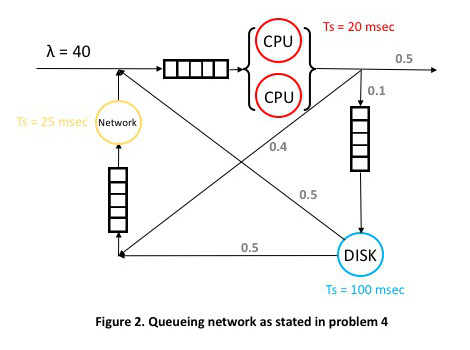
\includegraphics[scale = 0.5]{Figure2.jpg}
\end{center}
\item
Let the rate going through CPU be $x \text {   processes per second}$. From Figure 2 in part (a), we can find the following equation at steady state:\\
\begin{equation}x = 0.5x + 40\end{equation}
so $x = 80\text {   processes per second}$ = 0.08\text {   processes per msec}.\\
Now we can find:\\
\begin{align*}
  \rho_{CPU} &= \frac{1}{2}\lambda_{CPU}T_s(CPU) = \frac{1}{2}(0.08\text {   processes per msec})(20\text {   msec/process}) = 0.8\\
  \rho_{DISK} &= \lambda_{DISK}T_s(DISK) = (0.1)(0.08\text {   processes per msec})(100\text {   msec/process}) = 0.8\\
  \rho_{Network} &= \lambda_{Network}T_s(Network) = [(0.4)(0.08 + (0.1)(0.08)(0.5)]\text {   processes per msec}(25\text {   msec/process}) = 0.9\\
q_{CPU} &= \frac{\rho_{CPU}}{1-\rho_{CPU}} = 4\\
q_{DISK} &= 4. \\
q_{Network} & = 9
\end{align*} 
so the total response time: $$T_q = \frac{q_{total}}{\lambda} = \frac{4+4+9}{0.04} = 425 \text {   msec}$$\\

\item
In this problem, since the Network has the highest utilization among all the resources and it is likely to hit 100\% first, then the bottle-neck service unit is Network 
\item
Even though the CPU has dual-core, this system is limited by how much CPU can process. If the process rate were to increase above 50 processes per second, then the new rate going through CPU will be more than 100 processes per second, making the utilization of CPU per core more than 1. The result having utlization more than 1 would mean the queue will build up (for the demand is more than what the CPU can handle) to infinity. 
\end{enumerate}
\end{document}